\documentclass[12pt]{report}
\usepackage{graphicx}
\usepackage[utf8]{inputenc}
\usepackage[spanish]{babel}
\usepackage{setspace}
\usepackage{geometry}
\usepackage{titlesec}
\usepackage{times}
\usepackage{mathptmx} % Use mathptmx instead of times
\usepackage{fancyhdr}
\usepackage{float}



% Configuración de márgenes
\geometry{
    top=2.5cm,
    left=3cm,
    right=3cm,
    bottom=2.5cm
}

% Configuración de interlineado
\onehalfspacing

% Configuración de títulos y subtítulos
\titleformat{\chapter}[display]
  {\normalfont\bfseries\centering}{}{0pt}{\fontsize{14}{16}\selectfont}
\titleformat{\section}
  {\normalfont\bfseries}{\thesection}{1em}{\fontsize{12}{14}\selectfont}
\titleformat{\subsection}
  {\normalfont\bfseries}{\thesubsection}{1em}{\fontsize{12}{14}\selectfont}


% Configuración de pie de página
  \fancyhf{}
\fancyfoot[R]{\thepage}
\pagestyle{fancy}
\fancypagestyle{plain}{
  \fancyhf{}
  \fancyfoot[R]{\thepage}
}

  \begin{document}
  \pagenumbering{roman}
%----- PORTADA ----
\setlength{\hoffset}{27 pt} % 1 (Para centrar más la portada)
\begin{titlepage}
{\centering
{\fontfamily{ptm}\scshape\bfseries\fontsize{29.16}{34.992}\selectfont Universidad de Guadalajara \par}
\vspace{0.5cm}
{\scshape\Large Centro Universitario de los Lagos \par}
\vspace{1cm}
{\scshape\Large División de Estudios de la Biodiversidad e innovación Tecnológica \par}
\vspace{1cm}
{\graphicspath{{imagenes/Portada}} %ruta de las imagenes

\includegraphics[width=0.3\textwidth]{image.png}\par}
\vspace{1cm}
% Título
{\scshape\large\bfseries Practica 3 \par}
\vspace{1.5cm}
% Materia
{\large \textbf{Asignatura:} \\Sistemas Embebidos\par}
\vfill
% Estudiante
{\large \textbf{Presenta:} \\Oscar Iván Moreno Gutiérrez \#220942754
\\Arnold Jonathan Bradley Mercado Plascencia \#220942835
\\Alejandro Orozco Ramirez \#217490257  \par}
\vfill
% Profesor
{\large \textbf{Profesor:} \\Dr. Afanador Delgado Samuel Mardoqueo \par}
\vfill
\vfill
% Fecha
\begin{flushright}
  {\normalsize \textbf {Fecha:} \\ \today}
\end{flushright}
\vfill}
{\large  \par}
\end{titlepage}
%----- FIN DE PORTADA ----

%----- ÍNDICE GENERAL ----
\tableofcontents
\newpage

%----- PALABRAS CLAVE ----
\pagenumbering{arabic}
\chapter*{Palabras Clave}
\addcontentsline{toc}{chapter}{Palabras Clave}
\begin{itemize}
  \item ssh: secure shell
  \item ls: list
  \item pwd: print working directory
  \item cd: change directory
  \item sudo: super user do
  \item terminal: consola donde se ingresan comandos
\end{itemize}
\newpage

%----- OBJETIVO ----
\chapter*{Objetivo}
\addcontentsline{toc}{chapter}{Objetivo}
Identificar los formatos de los comandos del SO Linux en un hardware embebido de Raspberry Pi.
\begin{figure}[H]
  \centering
  
\includegraphics[width=0.5\textwidth]{Screenshots/piOS.png}
  \caption{Distribución de Linux en Raspberry Pi.}
  \label{fig:piOS}
\end{figure}
Pi OS es una distribución de Linux basada en Debian, diseñada para Raspberry Pi. Es un sistema operativo de código abierto que se puede descargar e instalar de forma gratuita.
\newpage

%----- CONTENIDO ----
\chapter{Contenido}
\section{Material}
\begin{itemize}
  \item Raspberry Pi 4
  \item Fuente de alimentación
  \item Cable micro HDMI a HDMI
  \item Monitor
  \item Teclado
  \item Mouse
  \item Conexion a traves del protocolo IP
\end{itemize}
\section{Procedimiento}
Ingresamos a la terminal de la Raspberry Pi, una vía remota a través de la IP de la tarjeta, y otra a través del HDMI conectado a un monitor. La conexión al monitor se hizo para verificar los cambios desde la tarjeta.
\begin{figure}[H]
  \centering
  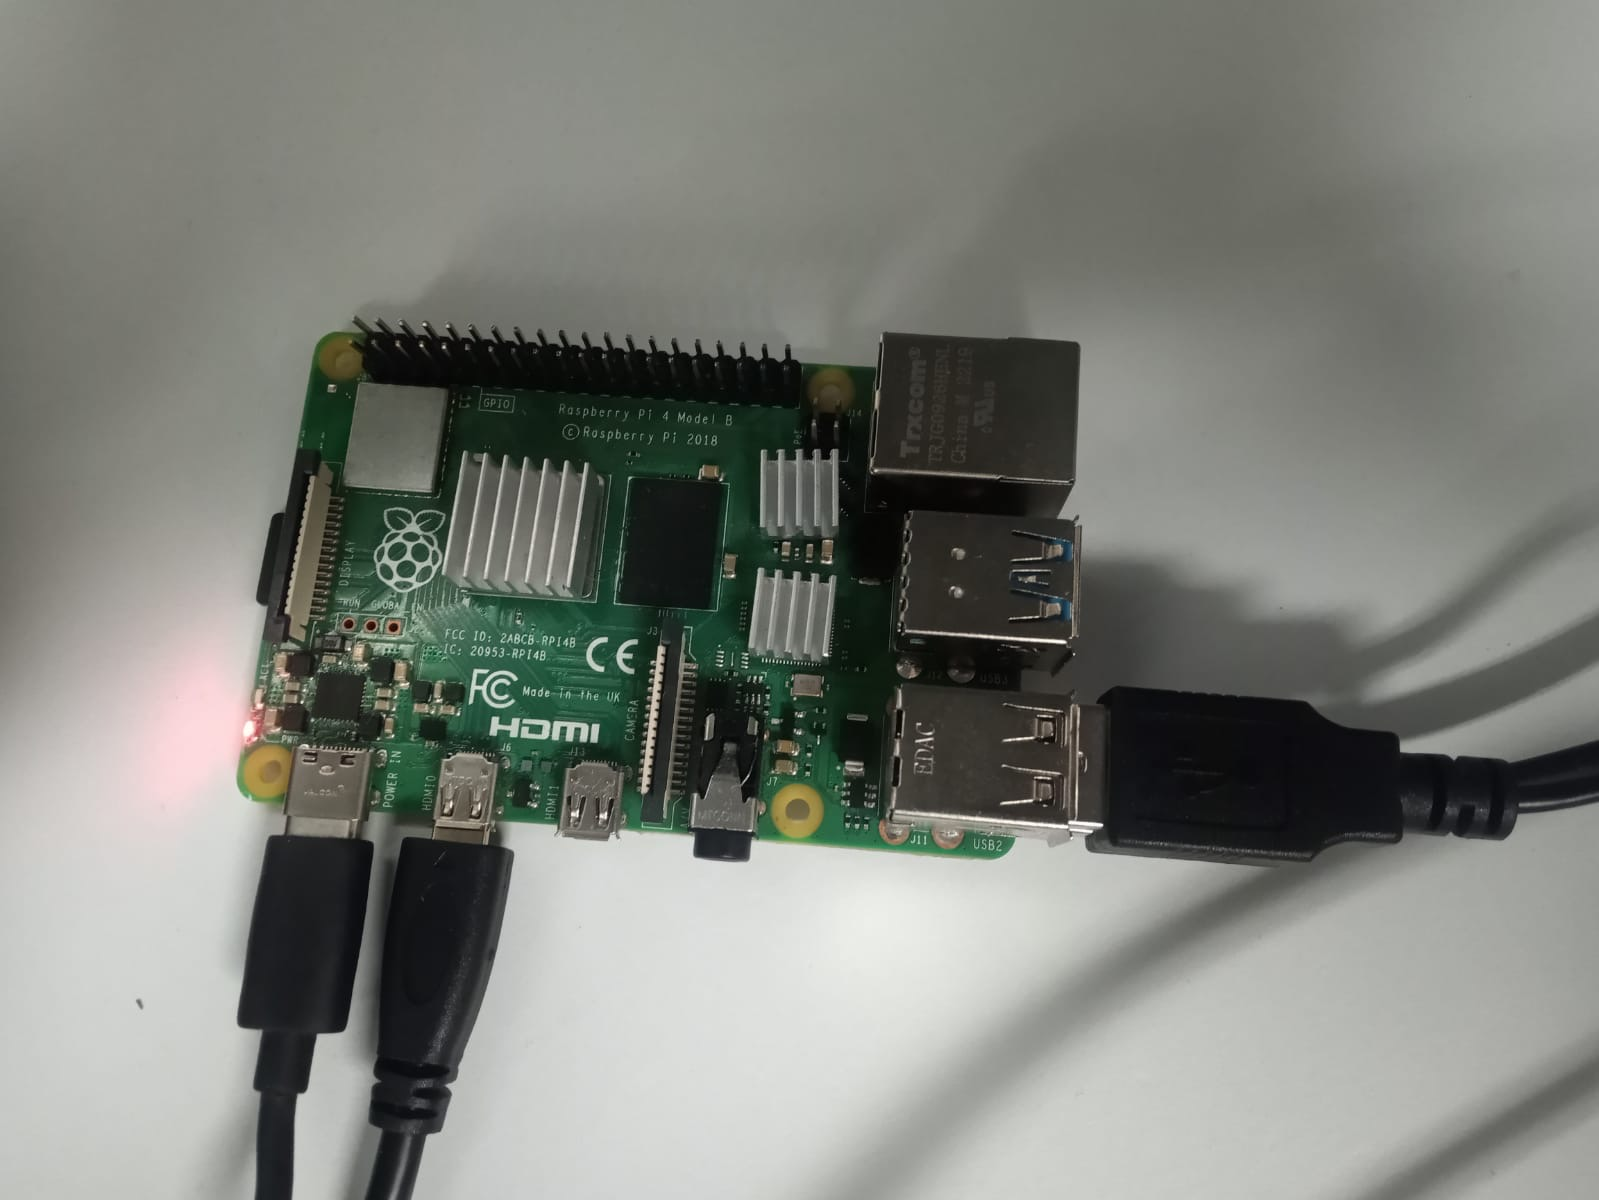
\includegraphics[width=0.5\textwidth]{Screenshots/raspberryPi.JPG}
  \caption{Raspberry Pi 4 y sus conexiones HDMI, USB para teclado, mouse y monitor.}
  \label{fig:raspberryPi}
\end{figure}
Ingresando a la terminal el comando ssh de la siguiente manera:
\begin{verbatim}
$ ssh rasPutin@rasPutin.local
\end{verbatim}
Luego nos pidió la contraseña de la tarjeta.
\begin{figure}[H]
  \centering
  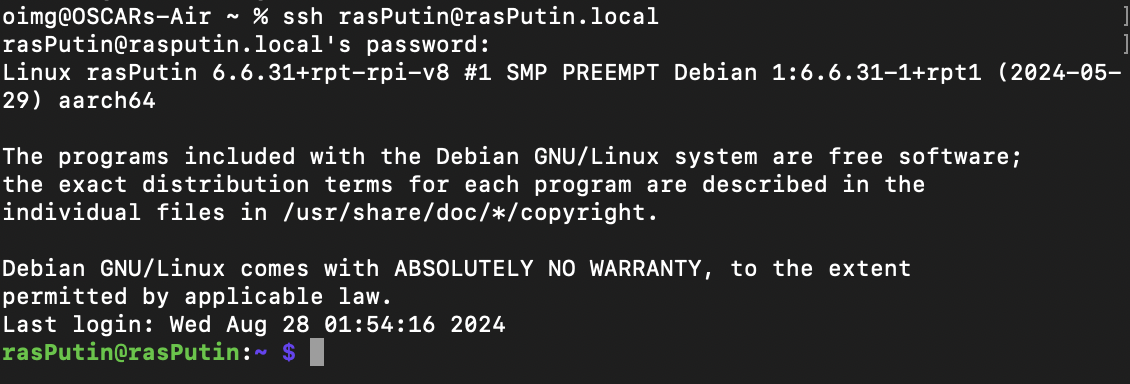
\includegraphics[width=0.5\textwidth]{Screenshots/ssh.png}
  \caption{Conexión a través de la IP de la tarjeta.}
  \label{fig:ssh}
\end{figure}

Listo, estamos conectados a la tarjeta a través de la IP.

Ahora vamos a ingresar comandos de Linux en la terminal de la Raspberry Pi.

Se ingresó ls y ls -al:
\begin{verbatim}
  $ ls
  $ ls -al
\end{verbatim}
Nos mostró los archivos y carpetas que se encuentran en el directorio actual. -al nos muestra los archivos ocultos y los permisos de los archivos y carpetas.
\begin{figure}[H]
  \centering
  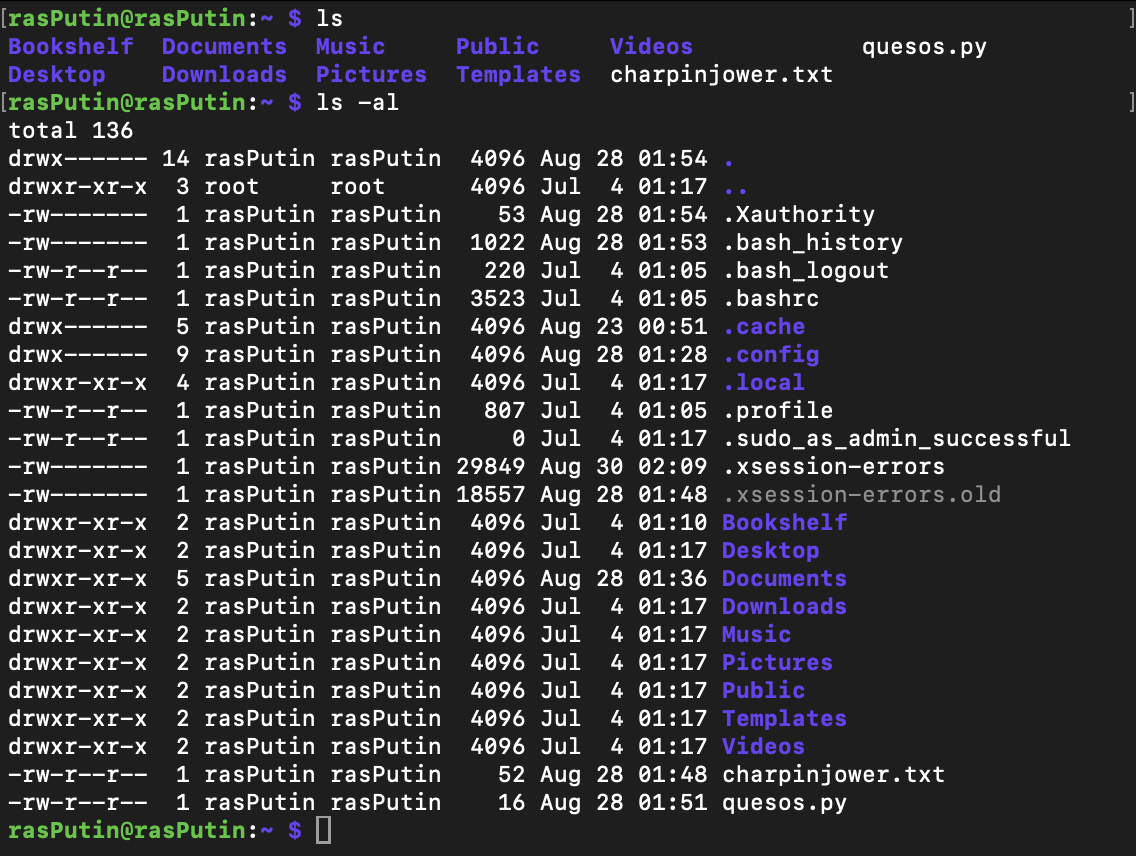
\includegraphics[width=0.5\textwidth]{Screenshots/ls.png}
  \caption{Comando ls y ls -al.}
  \label{fig: ls}
\end{figure}
Se ingresó pwd:
\begin{verbatim}
  $ pwd
\end{verbatim}
Nos muestra la ruta del directorio actual.
\begin{figure}[H]
  \centering
  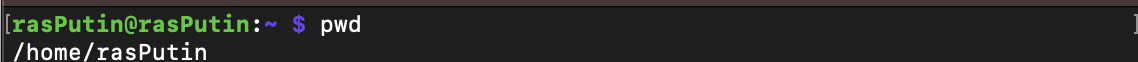
\includegraphics[width=0.5\textwidth]{Screenshots/pwd.png}
  \caption{Comando pwd.}
  \label{fig:pwd}
\end{figure}
Se ingresó cd:
\begin{verbatim}
  $ cd 
  $ cd /
\end{verbatim}
Ingresando el comando cd sin argumentos nos lleva al directorio home, y cd / nos lleva al directorio raíz.
\begin{figure}[H]
  \centering
  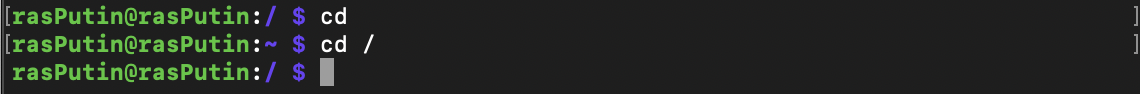
\includegraphics[width=0.5\textwidth]{Screenshots/cd.png}
  \caption{Comando cd y cd /.}
  \label{fig:cd}
\end{figure}

Podemos apagar la tarjeta con el comando:
\begin{verbatim}
  $ sudo shutdown -h now
\end{verbatim}
Aquí se muestra de la siguiente manera desde la terminal de la computadora conectada remotamente:
\begin{figure}[H]
  \centering
  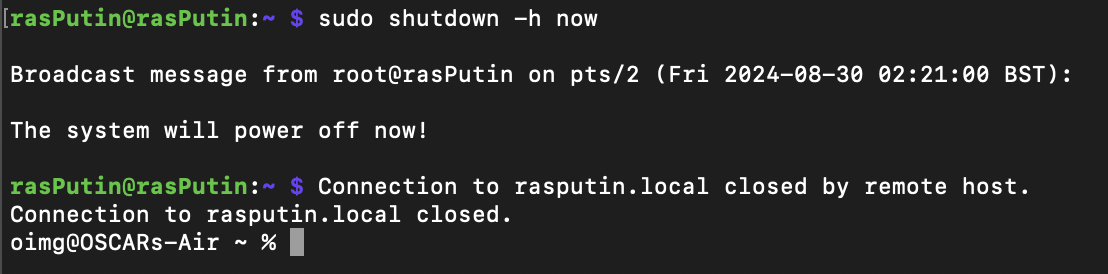
\includegraphics[width=0.5\textwidth]{Screenshots/apagando.png}
  \caption{Comando para apagar la tarjeta.}
  \label{fig:apagar}
\end{figure}

\section{Preguntas}
¿Cuál es el contenido del directorio /?

Primero vamos al directorio raíz con el comando cd / y luego ingresamos el comando ls para ver el contenido del directorio raíz.
\begin{verbatim}
  $ cd /
  $ ls
\end{verbatim}
\begin{figure}[H]
  \centering
  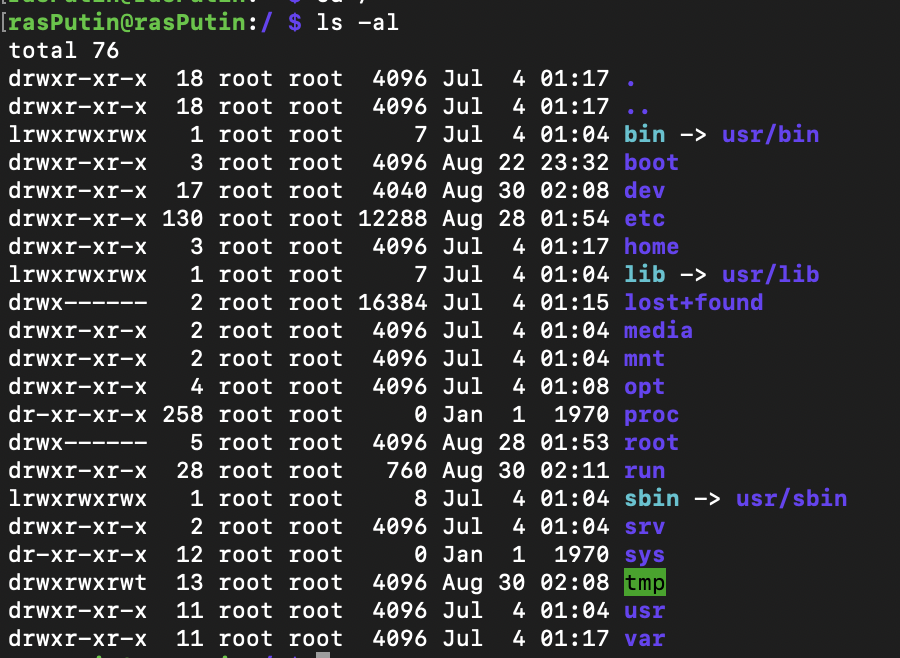
\includegraphics[width=0.5\textwidth]{Screenshots/contenidoRaiz.png}
  \caption{Contenido del directorio raíz.}
  \label{fig:raiz}
\end{figure}

¿Cuál es la ruta del directorio /?
Estando en el directorio raíz, ingresamos el comando pwd.
\begin{verbatim}
  $ pwd
\end{verbatim}
\begin{figure}[H]
  \centering
  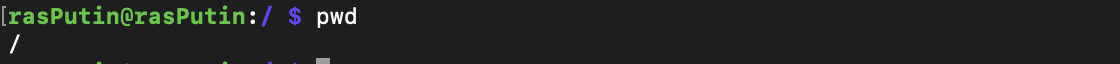
\includegraphics[width=0.5\textwidth]{Screenshots/rutaRaiz.png}
  \caption{Ruta del directorio raíz.}
  \label{fig:pwdRaiz}
\end{figure}

¿Qué comandos utilizarías para regresar al directorio inicial?
El comando cd sin argumentos o cd ~ nos lleva al directorio home.
\begin{verbatim}
  $ cd ~
  $ pwd
\end{verbatim}
\begin{figure}[H]
  \centering
  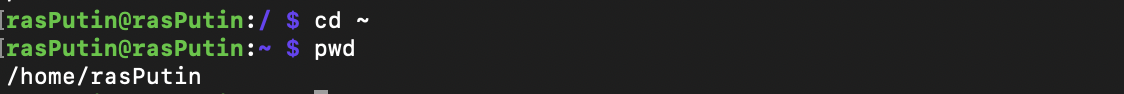
\includegraphics[width=0.5\textwidth]{Screenshots/regrsoHome.png}
  \caption{Comando cd \~~}
  \label{fig:cdHome}
\end{figure}
\newpage

%----- CONCLUSIONES ----
\chapter{Conclusiones}
Los comandos basicos de Linux son muy utiles para navegar por los directorios y archivos de la tarjeta Raspberry Pi, ademas de poder apagar la tarjeta de forma segura.
\newpage


\end{document}